% This is samplepaper.tex, a sample chapter demonstrating the
% LLNCS macro package for Springer Computer Science proceedings;
% Version 2.21 of 2022/01/12
%
\documentclass[runningheads]{llncs}
%
\usepackage[T1]{fontenc}
\usepackage{float}
% T1 fonts will be used to generate the final print and online PDFs,8;9M
% so please use T1 fonts in your manuscript whenever possible.
% Other font encondings may result in incorrect characters.
%
\usepackage{graphicx}
% Used for displaying a sample figure. If possible, figure files should
% be included in EPS format.
%
% If you use the hyperref package, please uncomment the following two lines
% to display URLs in blue roman font according to Springer's eBook style:
%\usepackage{color}
%\renewcommand\UrlFont{\color{blue}\rmfamily}
%
\usepackage{listings}
\usepackage{verbatim}
% Used for making  comments. 
\usepackage{placeins}
% If you use a FloatBarrier to prevent figures sliding to unwanted sections.

\usepackage{todonotes}

\begin{document}
%
\title{Ontology-Based Models of Chatbots for Populating Knowledge Graphs}
%
%\titlerunning{Abbreviated paper title}
% If the paper title is too long for the running head, you can set
% an abbreviated paper title here
%
\author{Petko Rutesic\inst{1}\orcidID{0000-0001-7017-707X} \and
Dennis Pfisterer\inst{2}\orcidID{0000-0002-4877-1088} \and
Stefan Fischer\inst{2}\orcidID{0000-0003-1292-8925}\and
Heiko Paulheim\inst{3}\orcidID{0000-0003-4386-8195}
}


%
\authorrunning{Rutesic et al.}
% First names are abbreviated in the running head.
% If there are more than two authors, 'et al.' is used.
%
\institute{Baden-Wuerttemberg Cooperative State University, 68163 Mannheim, Germany \and
  Institute of Telematics, University of Luebeck, Luebeck, Germany \and
  University of Mannheim, Mannheim, Germany 
}
%
\maketitle              % typeset the header of the contribution
%
\begin{abstract}
Knowledge graphs and graph databases are nowadays extensively used in various domains. However, manually creating knowledge graphs using existing ontology concepts presents significant challenges.  On the other hand, chatbots are one of the most prominent technologies in the recent past. In this paper, we explore the idea of utilizing chatbots to facilitate the manual population of knowledge graphs. To implement these chatbots, we generate them based on other special knowledge graphs that serve as models of chatbots. These chatbot models are created using our modelling ontology (specially designed for this purpose) and  ontologies from a specific domain.  The proposed approach enables the manual population of knowledge graphs in a more convenient manner through the use of automatically generated conversational agents based on our chatbot models.

\keywords{modelling  \and ontology \and chatbots \and knowledge graphs}
\end{abstract}
%
%
%
\section{Introduction}

Creating user-friendly interfaces to facilitate populating knowledge graphs manually is a very demanding task. In order to create a knowledge graph, it is necessary to have expertise not only in the domain of interest but also in the field of ontology engineering. We can illustrate this using an example of flight registration, where the end-users enter flight information manually in the knowledge graph and  the ultimate output of the process would be a comprehensive knowledge graph representing all existing flights. To define a specific flight, it is necessary to first choose the appropriate ontology for flight description and then create an individual of the class representing flights. Following that, the user has to know how to define departure and arrival airports, which requires the knowledge of object and data properties that can be used to describe airports. What makes this task even more complex is the need to choose whether these airports can be described as blank nodes or not, or to choose specific ontology design patterns. Creating these ontologies (editing RDF graphs) using only text editors in any syntax for representing RDF graphs would be intimidating for the majority of users.

Tools for ontology engineering like Protégé, WebProtégé, TopBraid Composer and similar tools are frequently used for this purpose. Additionally, there are various approaches to modelling user interfaces for populating knowledge graphs. These user interfaces are of different kinds, from desktop and web applications to conversational agents (chatbots). Particularly, chatbots have seen great growth in popularity, especially in the last couple of years with the appearance of large language models and tools like ChatGPT that use deep learning models to generate correct humanlike responses. Chatbots are now integrated in various domains and have numerous applications, such as e-customer care services, e-commerce systems, the medical field, etc.

Our approach aims to empower end users to create knowledge graphs like the aforementioned flight knowledge graph in a simple manner. The chatbot should primarily ask simple questions like: ``What is the flight number?'' or ``What is the flight destination?''. To this end, we propose to divide population of knowledge graphs in two processes. The first process would be modelling and designing of conversational agents, and the second process is using those conversational agents by many end users to populate desired knowledge graphs. One potential group of end users who could benefit from our chatbots includes airline personnel (or flight operators) responsible for registering new flights and services related to those flights. The novelty of our idea lies in the automatic generation of chatbots from models that themselves are knowledge graphs. By adopting this approach, the design of our conversational agent models becomes the responsibility of ontology experts (chatbot model designers), whereas the end users of the chatbots would not necessarily need expert knowledge in ontologies. This way, the end user would be relieved from the burden of precisely knowing domain ontologies and the intricacies of ontology engineering.

Our approach can be simply expressed through two functions. The first function is named the modelling function, which encompasses the process of modelling chatbot dialogues (conversations) while simultaneously defining the structure of the output knowledge graphs. The modelling function takes a set of domain ontologies and our $OBOP$ ontology (Ontology for Ontology-based Ontology Population) as input parameters. The $OBOP$ ontology is specifically designed for modelling purposes and can be accessed at \url{http://purl.org/net/obop} or in the GitHub repository\footnote{\url{https://github.com/ontosoft/logic-interface/blob/main/ontology/obop.owl}}.
$$ f_{modelling}(DomainOntologies, OBOP) = ChatbotModel$$
The modelling process is the task for chatbot model designers (ontology experts), and the output of this process is a $ChatbotModel$, which is a knowledge graph defined using elements from $DomainOntologies$ and our $OBOP$ ontology. Currently, the modelling is done manually, but we have plans to design special GUI tools to support and automate this process in the future.  

The second function represents the process of data acquisition, i.e., knowledge graph population. This process is actually the use of chatbot to enter data.
$$f_{acquisition}(ChatbotModel, UserInteraction) = OutputKnowledgeGraph$$
The acquisition function takes a chatbot model created in the modeling process and user interaction (during which the data is entered) as input parameters. The output of the acquisition function is a desired knowledge graph, referred to as $OutputKnowledgeGraph$, which is defined only using elements from the domain ontologies. In Figure~\ref{fig:chatbotsystem}, part of our approach that corresponds to the acquisition function is outlined. The \textit{Chatbot generator} takes the \textit{chatbot model} defined by elements of the OBOP ontology (colored in red) and domain ontologies (colored in black). The \textit{output knowlege graph} is populated through the interaction of the end-user with the chatbot and contains only elements from domain ontologies.
\begin{figure}[H]
  \centering
  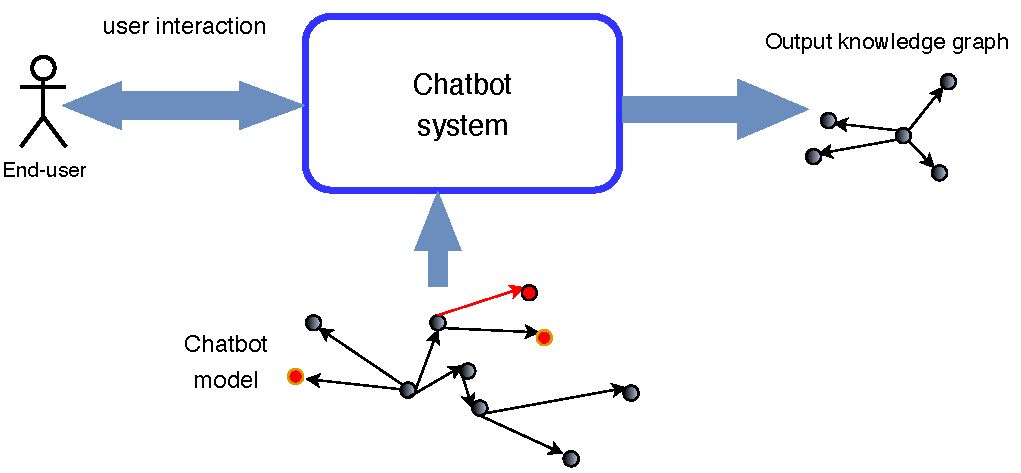
\includegraphics[width=0.9\linewidth]{img/chatbot-system}
  \caption{A simplified representation of the acquisition function}
  % \Description{Big picture }
  \label{fig:chatbotsystem}
\end{figure}
Since the main goal is to simplify the population of knowledge graphs using conversational systems (chatbots), we have explored the idea of modelling these chatbots also within knowledge graphs. To leverage the reasoning capabilities of OWL ontologies, it is reasonable for the chatbot models to be represented in the OWL DL ontology class. Therefore, the goal of our approach can be boiled down to the following set of requirements:
\begin{enumerate}
\item
  The chatbot conversation and the structure of the output knowledge graph are both specified within the same knowledge graph (e.g. RDF file), representing a model.
\item
  Models are defined using a dedicated ontology designed for this purpose, serving as a meta-model for generating our models.
\item
The meta-model comprises elements capable of modelling main program control structures, i.e., sequential, selection (branching) and iteration control structures. 
\end{enumerate}
\begin{comment}
The requirements to  this approach are that chatbot models should provide Turing completeness. Basic branching structures, loops has to be implemented in models. Models schould be general and therefore not tailored only for one domain, but applicable in arbitrary domains. Functionalities of chatbot modeling such as program flows should be modelled using knowldege graphs (ontology instances). Models are not overly complex for the implementation. In the next sections we explain how to implement these requirement..
\end{comment}
In the rest of the paper, we elaborate on the implementation of the proposed requirements. The rest of the paper is organized as follows: The next section presents a use case involving flight registrations, which will be used to illustrate our approach in subsequent sections. Then we describe the main elements of the OBOP ontology that model various aspects of chatbot conversations, and we showcase how the modelling function works on our use case with flight registrations. Each subsection focuses on specific workflows of the chatbot and explains how these workflows are modeled using entities from the OBOP ontology. Finally, the paper concludes with a section discussing the contributions of our work.
\section{Use Case}
To demonstrate the applicability of our chatbot models, we introduce an example involving a chatbot designed to help create knowledge graphs for flights. Essentially, we look at process from the reverse perspective, beginning with an existing knowledge graph and assuming it to be the output knowledge graph of a chatbot. Then we demonstrate a model of this chatbot that generates this particular knowledge graph. 

The knowledge graph that our chatbot has to construct is already presented in the examples of using the Ticket ontology\footnote{\label{Ticket Ontology}http://purl.org/tio/ns}. The authors of the knowledge graph used the GoodRelations ontology\cite{hepp2008goodrelations}, the Ticket ontology (compliant with GoodRelations) and DBpedia to decribe the flight. A simplified graphical representation of the flight knowledge graph is shown in Figure~\ref{fig:usecase}.
The flight knowledge graph contains data about a specific flight with the flight number LH1234, which is operated by Lufthansa airline. The flight information includes details about the departure and destination airports, as well as the types of tickets that can be booked for that flight. A flight ticket is defined as an instance of the class tio:Ticket of the Ticket ontology. In the graphical representation, individuals and blank nodes are depicted using circles, with blank nodes represented by empty circles. Ontology classes are illustrated by ovals, while data properties are shown as rectangles. 
\begin{figure}[H]
  \centering
  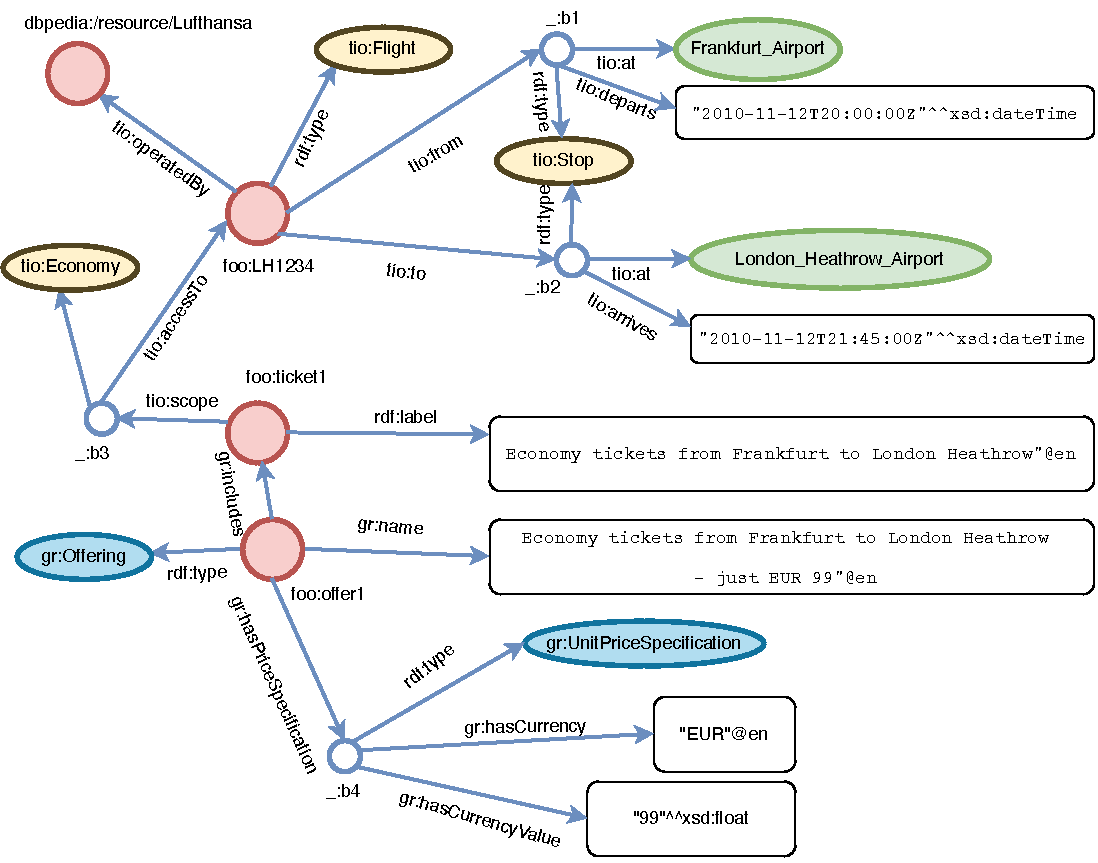
\includegraphics[width=\linewidth]{img/use_case}
  \caption{A knowledge graph representing a simple flight description.}
  % \Description{Big picture }
  \label{fig:usecase}
\end{figure}
\FloatBarrier
During the interaction with the chatbot, the user must provide the flight number, departure and destination airports, as well as the departure and arrival times.
Below is a representation of the example knowledge graph in RDF format using Turtle syntax, with the prefix definitions omitted for brevity:
\begin{lstlisting}[basicstyle=\small]
foo:LH1234 a tio:Flight ;
  tio:from [ a tio:Stop ;
     tio:at <http://dbpedia.org/resource/Frankfurt_Airport> ;
     tio:departs "2010-11-12T20:00:00Z"^^xsd:dateTime ] ;
  tio:to [ a tio:Stop ;
     tio:at <http://dbpedia.org/resource/London_Heathrow_
       Airport> ;
     tio:arrives "2010-11-12T21:45:00Z"^^xsd:dateTime ] ;
  tio:availableServiceLevel tio:Economy, tio:BusinessClass ;          
  tio:operatedBy  <http://dbpedia.org/resource/Lufthansa> .
            
foo:ticket5 a tio:TicketPlaceholder ;
  rdfs:label "Economy tickets from Frankfurt to
       London Heathrow"@en ;
  tio:scope [ a tio:ScopeOfAccess ;
     tio:accessTo foo:LH1234 ;
     tio:eligibleServiceLevel tio:Economy ] .

foo:HeppTickets gr:offers foo:offer1 .
foo:offer1 a gr:Offering ;
     gr:name "Economy tickets from Frankfurt to London
          Heathrow - just EUR 99"@en ;
     gr:description "Special Offer: Economy tickets from
          Frankfurt to London Heathrow for just EUR 99"@en ;
     gr:includes foo:ticket5 ;
     gr:eligibleRegions "DE"^^xsd:string ;
     gr:hasBusinessFunction gr:Sell ;
     gr:hasPriceSpecification
       a gr:UnitPriceSpecification ;
         gr:hasCurrency "EUR"@en ;
         gr:hasCurrencyValue "99"^^xsd:float ;
         gr:validThrough "2010-11-11T23:59:59"^^xsd:dateTime];
     gr:acceptedPaymentMethods gr:MasterCard, gr:VISA ;
     gr:availableDeliveryMethods tio:Etix .	
\end{lstlisting}
The knowledge graphs (instances of the Ticket ontology) generated using our chatbot offer significant usefulness as they can be easily searched by customers looking to book flight tickets. The use of ontologies in the system allows for defining search operations using SPARQL queries.
Moreover, customers have the option to employ conversational agents like KBot\cite{ait2020kbot} in order to find suitable flight tickets using natural language understanding over linked data. In that case semantic web technologies can be used directly to find suitable flights without resorting to web scraping methods as described in \cite{turnip2019application}.        

The primary objective of our chatbot use case is to simplify the process for end-users by posing straightforward questions, while the knowledge graph is generated seamlessly in the background using answers to those questions. The chatbot must have the capability to generate this knowledge graph and also to accommodate its extensions, such as adding the definition of additional ticket types if needed. By doing so, the chatbot determines the structure of the output ontology without explicitly asking the user to specify blank nodes, instances of specific ontology classes and other details, thereby alleviating the burden of detailed ontology engineering. To achieve this level of sophistication, the chatbot model incorporates all the necessary details, and the key aspects of the model are outlined in the section dedicated to modelling architecture.
\section{Related work}
One of the first known conversational agents is ALICE \cite{wallace2009anatomy} which uses AIML (Artificial Intelligence Markup Language) which is basically XML to design conversations. The system uses a botmaster which monitors conversations to make them more appropriate. Unlike writing rules in a XML based language, the rules in our approach are encoded in a knowledge graph based on our modeling ontology and can be stored in an RDF file. Historically, there have been various approaches to using semantic nets to generate chatbot. One of the first examples is OntBot \cite{al2011ontbot} that transforms ontologies and knowledge into relational database and then uses relational database to generate chats. Another example of usage of model-driven conversational systems is presented in \cite{perez2020model}, wherein a specialized domain-specific language with components like intents, entities, actions and flows is employed to design the dialogue structure of task-oriented chatbots. The dialog management used in our paper is also similar to the dialog management used by the Rasa chatbot \cite{bocklisch2017rasa}. However, our approach differentiates itself from those appraches by aiming to represent all components, including intents, flows and actions through the use of knowledge graphs. 

There have been many approaches to model user interfaces and web-application logic using knowledge graphs. An approach described in \cite{rutesic2021enhanced} proposes a method of modelling HTML application structure and its logic using RDF graphs.
In this paper, we deal with a similar question of modelling and generating chatbots used to engage in dialogs with users to acquire data. Furthermore, the acquired data is used to directly populate desired output knowledge graphs based on domain ontologies. The expressiveness of formal ontologies proves valuable in representing both the models of chatbots and the complex knowledge within the business logic of target ontologies.
Chatbots generated using this approach could prove advantageous wherever the description of complex products and services using ontologies is required, as is the case in emerging business models like {\itshape Distributed Market Spaces} \cite{radonjic2020arising}. This approach complements the method described in \cite{hitz2016generic}, where the system utilizes SPARQL queries to identify appropriate complex products and services.  

As stated in \cite{agarwal2020review}, conversational clients or chatbots are designed to be used either as task-oriented or open-ended dialog generators. In our approach, we develop a task-oriented chatbot responsible for collecting data (knowledge graph) based on particular ontologies. The actual task is described based on rules specified in the model represented again as knowledge graph defined using our OBOP ontology. Thus, our chatbot can also be classified as a rule-based chatbot. To enable human-like conversation, our task-based chatbot module is incorporated in a an open-ended chatbot which is further described in the implementation section. The intention of our system is not to design a chatbot capable of convincing a human that (s)he is chatting with a human instead of a computer program. That intelligent behavior depends on good knowledge sets. Instead, we focus on the creation of chatbots that gather information in the form of knowledge graphs with individuals (instances) of the respective domain ontologies.  



\section{Model architecture}
Our meta-model (OBOP ontology) contains various structures that describe chatbot functionalities. The fundamental structure is designed to specify a simple data request. In response to this request, the user inputs a value, which is then validated and can be stored in the system as a data property, IRI, or for a similar purpose. This functionality corresponds to the process of entering data into form fields in GUI interfaces. To represent the insertion of these data values, the OBOP ontology, uses an instance of the class obop:SingleValueRequest. In cases where multiple data properties need to be entered as a group of questions, this is modeled using a conversation block. The generation of chatbot models, using constructions explained in the next sections, is the responsibility of chatbot model designers.  

\subsection{Conversation block}
A conversation block represents a segment of a conversation used to collect data values which are frequently related to a specific entity. This part of the dialog is analogous to an HTML form in web applications. The chatbot poses a series of questions, and through providing answers to those questions, the system stores corresponding values. A simple model for entering the flight IRI is illustrated in Figure~\ref{fig:conv_block}. In this figure, blue circles represent instances of classes of the OBOP ontology, while slightly bigger peach-colored circles depict instances from domain (target) ontologies. Yellow ovals represent classes from the OBOP ontology, and blue ovals stand for the classes from the target ontology. Object and data properties are denoted by directed lines with labels that specify names of those properties.     

\begin{figure}[H]
  \centering
  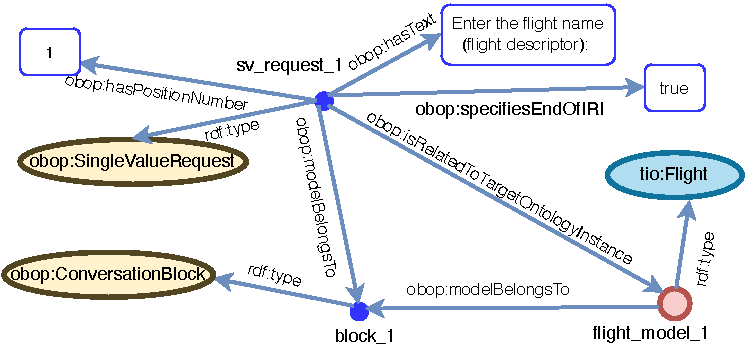
\includegraphics[width=\linewidth]{img/conversation_block}
  \caption{Modelling a block of conversation}
  % \Description{Modelling conversation block of the chatbot system }
  \label{fig:conv_block}
\end{figure}


A segment of the model represented in Figure \ref{fig:conv_block} should initiate the following part of conversation:
\begin{lstlisting}[basicstyle=\small,  xleftmargin=0.7cm ]
chatbot: Please enter the flight name (flight descriptor):
user:    LH1234
\end{lstlisting}
The outcome of the previous conversation is adding of the following triple to the output knowledge graph:
\begin{lstlisting}[basicstyle=\small,  xleftmargin=0.7cm ]
foo:LH1234 a tio:Flight. 
\end{lstlisting}
In Figure~\ref{fig:conv_block} can be seen a conversation block named \textit{block\_1}, which has one instance of the class obop:SingleValueRequest called \textit{sv\_request\_1}. This represents a question for entering a flight name (a unique flight descriptor). \textit{sv\_request\_1} has the object property obop:specifiesEndOfIRI, which has boolean value true. This indicates that the provided answer to the question serves as the ending part of IRI representing the flight instance. The model of the instance of tio:Flight class that will be generated in this process is represented by the \textit{flight\_model\_1} instance. During the conversation with the chatbot from this instance will be generated the instance with the name foo:LH1234. Should the inserted string need to be the value of a data property instead of being part of the IRI, this would be indicated by the \textit{obop:containsDatatype} object property of the \textit{sv\_request} instance which would specify the name of the wanted data property. The object property \textit{obop:isRelatedToTargetOntologyInstance} indicates what instance will be transformed with the entered data. The data property \textit{obop:hasPositionNumber} specifies that this question is the first one in this conversational block.  


\FloatBarrier
\subsection{Branching control structure}
To enable chatbot users to make decisions and select different paths of execution, the OBOP ontology has mechanisms for modeling branching control structures. The class \textit{obop:Branching} represents a conditional structure. A simple branching structure in our example is explained in the case of selecting an airline that operates the given flight. The chatbot user is therefore prompted to choose only one airline company from the presented options.  
One possible conversation is presented in the following listing:
\begin{lstlisting}[basicstyle=\small,  xleftmargin=0.7cm ]
chatbot: Enter the airline that operates your flight.
         Choose one of the following options:
         1. Lufthansa
         2. Ryanair
user:    Lufthansa 
\end{lstlisting}
The chatbot asks a question and specifies a list of possible options. The user responds by writing one among those listed names or by writing the ordinary number in front of the corresponding name. For the sake of brevity, we decided to present only two possible options (two airlines) to choose from. This statement is similar to the ''switch'' statement in programming languages. As the result of the execution of this part of the chatbot the output graph can be extended with the following triple:
\begin{lstlisting}[basicstyle=\small,  xleftmargin=0.7cm ]
foo:LH1234
  tio:operatedBy <http://dbpedia.org/resource/Lufthansa>.
\end{lstlisting}
The segment of the model that generates the previous chatbot question and adds the specified triple, as the consequence of the chosen option, is represented in Figure \ref{fig:branching_schema}. It can be observed that the previous conversational block \textit{block\_1} is used, as it is regarded a part of the same conversation section. The question to choose one out of several possible values is denoted by an instance of the obop:Question class, called \textit{question\_1}. \textit{question\_1} has the data property \textit{obop:hasText} with the text of the question. Additionally, the question has the value of 2 for the \textit{obop:hasPositionNumber} data property, that serves to denote that this question has second place in the conversation block.         
The question \textit{question\_1} has an instance of the class \textit{obop:hasBranching} called \textit{branching\_1} and this branching is specified by the instance of the \textit{obop:Connection} class named \textit{conn\_1}.
\begin{figure}[H]
  \centering
  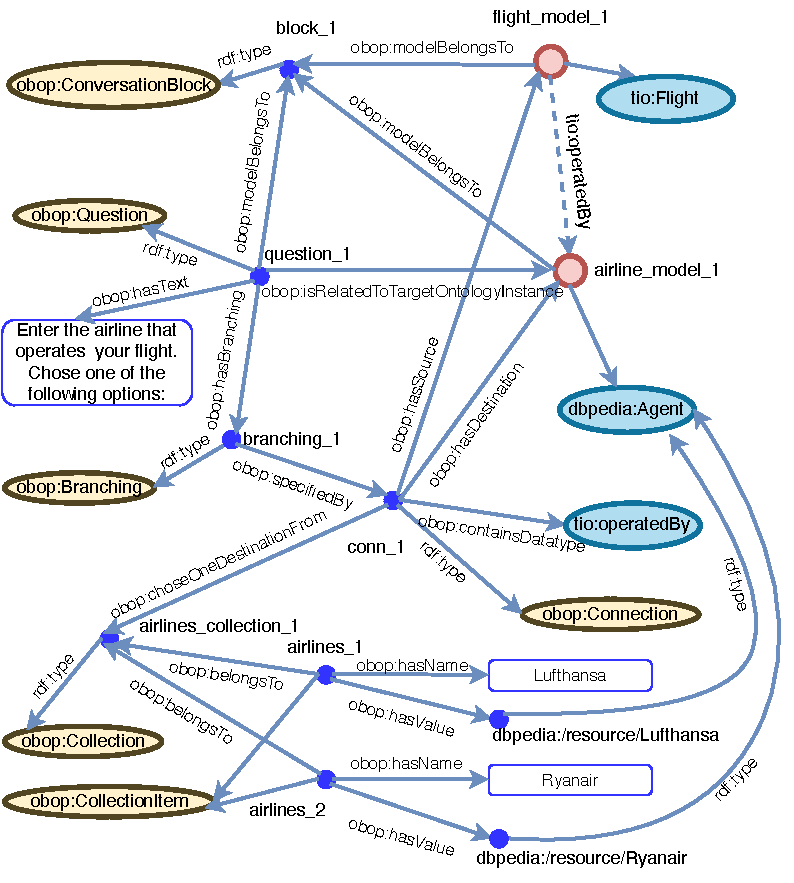
\includegraphics[width=\linewidth]{img/branching_schema}
  \caption{A part of the model specifying the process of selecting an airline}
  % \Description{Branching to decide on the operating airline}
  \label{fig:branching_schema}
\end{figure}

The obop:Connection class specifies how the two instances of the ontology classes should be related. An instance of this class has functional properties that specify source and destination of object properties. In our case, the source is an instance called \textit{flight\_model\_1} and the destination is \textit{airline\_model\_1}. The latter serves serves as a model for an instace of the  \textit{dbpedia:Agent} class, which will be created during the interaction with the chatbot. Additionally, the object property that has to be inserted in the output graph between these two instances is specified by the \textit{obop:containsDatatype} object property and it is, in our contex, \textit{tio:operatedBy} property. This particular object property is denoted by a dashed line in Figure \ref{fig:branching_schema}, although this edge is not part of the actual model graph.    

It can be seen that the connection instance specifies both a predicate (object property) and an object (instance) of a new triple. The user, interacting with the chatbot, is required to choose a single airline from the list of possible airlines. In the lower section of Figure \ref{fig:branching_schema} is defined an instance of the \textit{obop:Collection} class, named \textit{airlines\_collection\_1}. The connection instance conn\_1 is related to this collection by the object property \textit{obop:choseOneDestinationFrom}, which specifies exactly how to form the object of a new triple. In this case, our simple collection contains two instances of the class \textit{obop:CollectionItem} corresponding to Lufthansa and Ryanair airlines. 
OBOP collections are not defined using rdf:Bag, rdf:Seq or by using restrictions like \textit{owl:someValuesFrom}. Collections are basically used by the chatbot program in the runtime phase and they are not meant to be used in the process of ontology reasoning.     

An alternative, that can be specified in our model, which brings more generality to this example,  is to allow the user to directly input an IRI of the desired airline, which must belong to the \textit{dbpedia:Agent} class. However, we presented the selection from the list of available options to show that model designer has this option.

\FloatBarrier 
\subsection {Iteration control structure}
To effectively manage control flows, the chatbot model has to provide definition of iteration structurues (loops). As the iteration structures in programming languages allow the repetitive execution of a specific code block, iteration structures in chatbots enable the repetition of a set of questions within a conversation block or the repetition of other activities. For this purpose, the OBOP ontology introduces the \textit{obop:Loop} class. 

An example of iterations can be demonstrated within our flight scenario. The user has to define various ticket types for the flight, which could initiate the following conversation:
\begin{lstlisting}[basicstyle=\small,  xleftmargin=0.7cm ]
chatbot: Do you want to define one more ticket type?
user:    Yes
chatbot: Please enter the label of the ticket?
user:    Economy tickets from Frankfurt to London Heathrow
chatbot: Choose the service level of the ticket?
user:    Economy
chatbot: Do you want to define one more ticket type?
\end{lstlisting}
The result of executing the previous chatbot conversation is the following part of the graph:
\begin{lstlisting}[basicstyle=\small,  xleftmargin=0.7cm ]
foo:ticket5 a tio:TicketPlaceholder ;
  rdfs:label "Economy tickets from Frankfurt to London
             Heathrow"@en ;
  tio:scope [ a tio:ScopeOfAccess ;
     tio:accessTo foo:LH1234 ;
     tio:eligibleServiceLevel tio:Economy ] .
\end{lstlisting}
The part of the model that generates the preceding section of the chatbot conversation is illustrated in Figure \ref{fig:iteration_example}. The question \textit{question\_2} to ask for a new ticket type is related to an instance of the \textit{obop:Loop} class called \textit{loop\_1}. Each iteration of the loop specifies adding a new ticket which is represented by a conversational block \textit{block\_3}. If the user answers positively to the chatbot's question, a new ticket instance is generated according to the \textit{ticket\_model\_1}. Together with the ticket is generated a blank node corresponding to the \textit{\_:bnode} instance. The new blank node is related to the flight instance which is already created in the previous examples according to the \textit{flight\_model\_1}.
\begin{figure}[H]
  \centering
  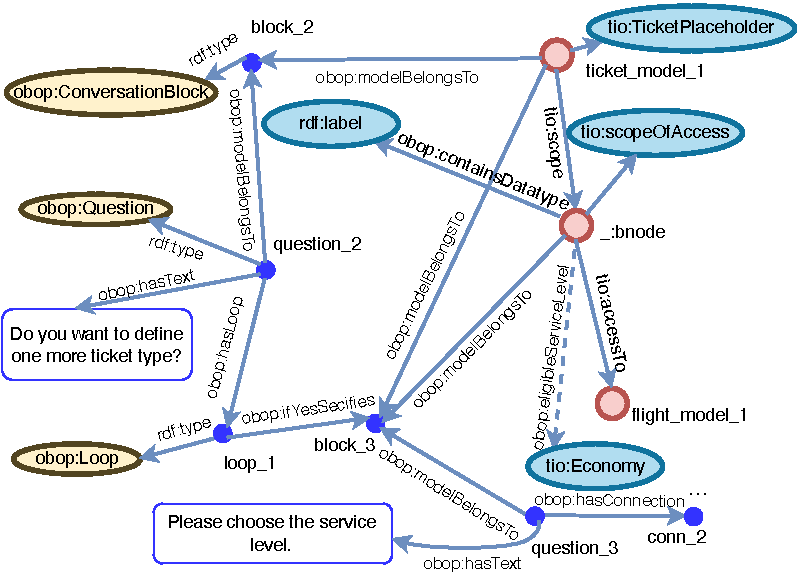
\includegraphics[width=\linewidth]{img/iteration_example}
  \caption{A part of the model used to define tickets using iteration.}
  % \Description{Iteration}
  \label{fig:iteration_example}
\end{figure}

The object properties \textit{tio:scope} and \textit{tio:accessTo} are also automatically created. However, \textit{rdfs:label} had to be specified using \textit{obop:containsDatatype} object property. In order to choose between possible service classes (e.g., Business or Economy) a new question (\textit{question\_3}) and connection (\textit{conn\_2}) was necessary. \textit{conn\_2} is not completely presented and ontology classes of same instances are omitted in Figure \ref{fig:iteration_example} for improved readability. 


\FloatBarrier 
\section {Implementation}
To implement a prototype of our chatbot, we employed Python libraries, namely, \textit{ChatterBot} as the conversational dialog engine and \textit{Owlready} \cite{lamy2017owlready} for ontology-oriented programming, to facilitate the creation and manipulation of OWL ontologies. The chatbot prototype can be tested as a REST application implemented using Flask framework\footnote{\label{flaskfootnote}https://flask.palletsprojects.com} with a simple JavaScript frontend. The source code can be found on Github\footnote{\url{https://github.com/ontosoft/ontochatbot}}. 

Chatbots generated using the ChatterBot library answer to user questions based on functionalities of logic adapters. For example, there are adapters like the \textit{Time adapter} that can answer question like `` What time is it?'', a the \textit{Math adapter} that can handle arithmetic operations, etc. When the user submits a question, all logic adapters assess whether they are capable of providing a response. The ability of a logical adapter to answer the question is measured by a confidence factor, expressed as a decimal value between 0 and 1. The answer from the adapter with the highest confidence is chosen as the reply. The architecture of our chatbot is shown in Figure~\ref{fig:architecture}.
\begin{figure}[H]
  \centering
  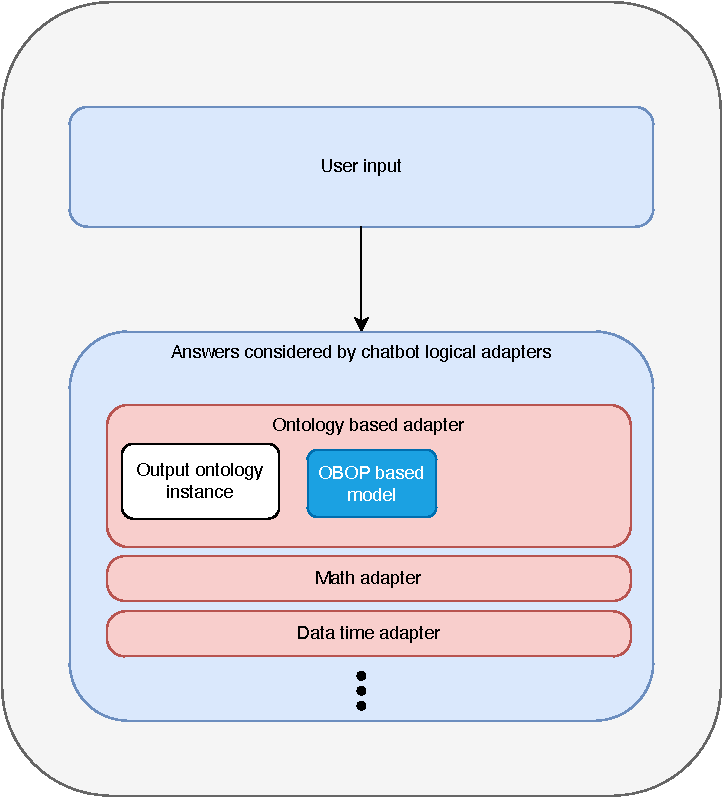
\includegraphics[width=0.5\linewidth]{img/architecture}
  \caption{Architecture of the chatbot system.}
  % \Description{Architecture o fthe chatbot sytem }
  \label{fig:architecture}
\end{figure}
Our model-based chatbot functionalities are implemented as a logic adapter for the ChatterBot library, named the \textit{OntoBasedAdapter}. Unlike other logic adapters in ChatterBot, the OntoBasedAdapter keeps track of the current state of conversation. Once the OntoBasedAdapter starts to gather information and populate the corresponding output knowledge graph, it needs to store information of the conversation's current state. It includes tracking visited nodes to enable system to make reverse steps and undo entries if necessary. Chatbot stores information on the current context, which is comprised of the entire array of nodes that have been visited and created during in the conversation up to the current state. 

Keeping track of the state of an ongoing dialogue is quite challenging task.
In the study \cite{altinok2018ontology}, authors dealt with this problem by exploiting ontologies for both knowledge base and the dialog manager in domain-driven conversation, creating a banking chatbot. Our chatbot, on the other hand, is a domain independent conversational agent, with the domain basically specified in the corresponding chatbot model. 

\subsubsection{Answering questions and generating replies}
When the OntoBasedAdapter takes charge of the dialog, it retains the conversation status. The system asks questions in the order that is defined by the chatbot model. If the user asks a question which is not related to the current task specified in the model and the conversation might take a different direction, potentially allowing another logic adapter to take charge and respond, enhancing the conversation's natural flow. Subsequently, it is posed a question by OntoBasedAdapter to pick up the conversation at the point where it was interrupted. This capability stems from the OntoBasedAdapter's management of context and conversation state.    
The confidence factor determines what logic adapter among all logical adapters will be chosen to give the answer. However, if the OntoBasedAdapter already started to gather information according to a conversation model then it has precedence over other logical adapters. Even if a user abruptly shifts the conversation's focus, the conversation agent tries to steer it back to the desired topic. For instance, if a user asks ``What time is it?'' during a conversation meant to schedule flight details,  the system employs the \textit{Time logic adapter} to answer promptly, before returning to the next question in line based on the chatbot model. 

In this way, each chatbot's response (question) is assigned with a corresponding weight (confidence factor). The challenges associated to this way of choosing replies include the fact that confidence factors of already implemented adapters tend to be quite high values. The solution which we use is that OntoBasedAdapter always returns confidence factor equal to 1 after it started to collect information. At present, responses are manually embedded into the model by the model designer.

\section{Contribution}
In this paper we introduced models for conversational agents (chatbots). These chatbots can accomplish domain-specific tasks such as generating flight descriptions, booking flight tickets or creation of restaurant menues that could be used for restaurant reservations in a user-friendly manner.  
In order to show how to create a chatbot model, we designed a chatbot intended for flight descriptions. 
The chatbots we propose adhere to the rule-based chatbots, where replies are generated using predefined rules intgerated in the models of respective conversations. These conversation models represent templates according to which replies (questions) are created.   

The requirements to the approach outlined in the introduction of the paper are met with our implementation. The conversation model and the structure of the knowledge graph are both included in the same knowledge graph according to the first requirement. The limitations of this approach are high complexity of the model graphs and challenging maintenance of the generated graphs. The second and third requirements are addressed by the explicit definition of specific classes, object properties, and data properties in the OBOP ontology. These definitions correspond to fundamental programming control structures, ensuring the capability to capture and manage various aspects of the conversation's flow and logic. 

Describing chatbot models based on OWL ontologies might offer significant benefits, including the potential for OWL reasoning applied to these models. The OWL reasoning capability could identify flawed models that might result in inconsistent knowledge graphs. Another advantage lies in the potential for reusing existing models, enabling their sharing and querying through SPARQL. Moreover, the application of machine learning algorithms to existing models could streamline the process of automatically or semi-automatically generating new chatbots for description of similar problems.

\begin{comment}
  
The user has an aim to get an information and to accomplish a goal. In our case the ontology model is used to conclude what the chatbot should say next. 
Chatscript can use Wordnet ontologies to improve responses.

OpenCyc [20] and Wordnet [21] 

We start presenting the review of literature that considers using ontologies and chatbots. 

An example which illustrates how our modelling works is a definition of a simple flight itinerary for a flight booking. \verb|https://www.chegg.com/homework-help/questions-and-answers/flight-ontology-online-travel-portal-engaged-well-known-airline-develop-ontology-support-i-q86451860| 
\end{comment}

%
% ---- Bibliography ----
%
% BibTeX users should specify bibliography style 'splncs04'.
% References will then be sorted and formatted in the correct style.
%
\bibliographystyle{splncs04}
\bibliography{mybibliography}
%
\end{document}
